
% ==============================================================================
\chapter{Detalhamento de trabalho}

Nesse capítulo, apresentaremos a arquitetura da plataforma Android, assim como o
ciclo de vida de uma aplicação para essa plataforma. Por fim, discutiremos os 
mecanismos de controle das variabilidades.

 Estudo das variabilidades da plataforma
 Mecanismos de controle
 Exemplos do Estudo de caso, quando possível

% ------------------------------------------------------------------------------
\section{Plataforma Android}
Segundo \cite{whatisandroid}, o Android é uma pilha de software para dispositivos
móveis que inclui um sistema operacional, middleware e aplicações chaves. O Android
SDK fornece as ferramentas e API's necessários para o desenvolvimento de aplicações
para a plataforma, utilizando a linguagem de programação Java.

\subsection{Características}
\begin{itemize}
    \item Framework de aplicações: permite o reuso e troca de componentes.
    Os desenvolvedores têm acesso completo à mesma API que é usada pelas aplicações
    do núcleo da plataforma.
    \item Máquina virtual Dalvik: é uma máquina virtual especializada para o uso em
    dispositivos móveis. Aplicações escritas em Java são compiladas em bytecodes para
    essa máquina virtual, e não uma máquina virtual Java.
    \item Navegador integrado: navegador baseado no motor {\it open source} WebKit
    \item Otimizações gráficas: possibilitadas por uma biblioteca gráfica 2D 
    personalizada; gráficos 3D baseadas na especificação OpenGL ES 1.0 (acelaração
    por hardware opcional)
    \item SQLite: para armazenamento de dados estruturados
    \item Suporte para multimídia: suporte para os formatos mais comuns de 
    áudio, vídeo e imagem (MPEG4, H.264, MP3, AAC, AMR, JPG, PNG, GIF)
    \item Rico ambiente de desenvolvimento: incluindo um emulador de dispositivo,
    ferramentas para depuração, {\it profiling} de memória e perfomance, e um {\it plugin}
    para o Eclipe IDE
    \item Alguns recursos dependentes do dispositivo
        \begin{itemize}
            \item Telefonia GSM 
            \item Bluetooth, EDGE, 3G, e WiFi
            \item Camera, GPS, bússola, e acelerômetro
        \end{itemize}
\end{itemize}

\subsection{Arquitetura da plataforma}

A figura \ref{system-architecture} mostra os principais componentes do sistema 
operacional Android. Cada seção é descrita abaixo.

\begin{figure}[h]
    \centering
    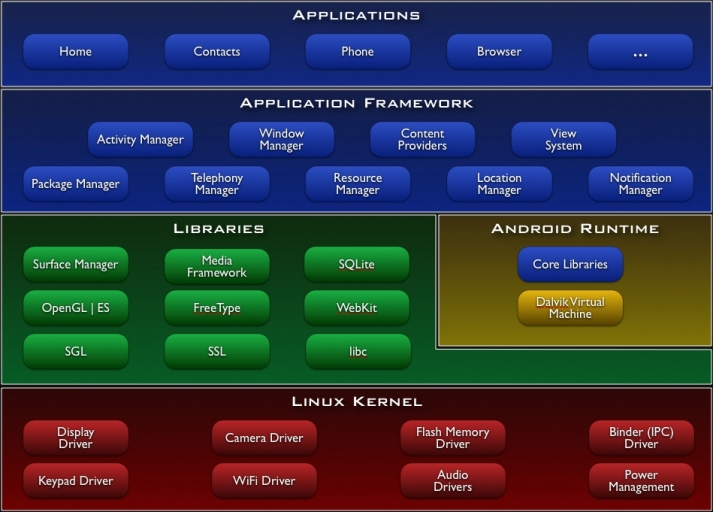
\includegraphics[width=10cm]{img/system-architecture.jpg}
    \caption{Arquitetura da plataforma Android}
    \label{system-architecture}
\end{figure}

\subsubsection{Application}
Android será distribuido com um conjuto de aplicações centrais, incluindo um cliente
de e-mail, programa de SMS, calendário, mapas, navegador, entre outros. Todas as 
aplicações são escritas em Java.

\subsubsection{Application Framework}
Fornecendo uma plataforma de desenvolvimento aberta, Android permite aos desenvolvedores
criarem aplicações extremamente ricas e inovadores. Desenvolvedores são livres para
tirar vantagem do hardware dos dispositivos, acessar informações de localização, 
executar serviços em backgrounds, definir alarmes e notificações para a barra de 
status etc.

Desenvolvedores tem total acesso às mesmas API's do framework usadas pelas aplicações 
do núcleo. A arquitetura da aplicação é projetada para simplificar o reuso de componentes;
qualquer aplicação pode publicar suas capacidades(?) e qualquer outra aplicação pode 
fazer uso dessas capacidades (sujeito às restrições de segurança impostas pelo 
framwork). Esse mesmo mecanismo permite que componentes sejam substituídos pelo 
usuário.

Os principais componentes do Application Framework são:
\begin{itemize}
\sloppy % evita que em linhas muito longas o espaço entre as palavras seja
        % aumentado
    \item System View: uma 'view' representa um widget que aparece na tela
    \item Content Providers: permite que aplicações possam acessar dados de outras 
    aplicações, ou compartilhar seus dados com outras
    \item Resource Manager: fornece acesso para recursos que não são código, como 
    strings de localização, gráficos e arquivos de layout
    \item Notification Manager: permite que as aplicações exibam alertas customizados 
    na barra de status
    \item Activity Manager: gerencia o ciclo de vida das aplicações e fornece um 
    mecanismo comum de navegação
\fussy % dual do \sloppy
\end{itemize}

\subsubsection{Libraries}
Android inclui um conjunto de bibliotecas C/C++ usada por vários componentes do 
sistema. Esses recursos são expostos para os desenvolvedores através do "application 
framework". Algumas das principais bibliotecas são listadas a seguir:

\begin{itemize}
    \item System C library - implementação da bibliotec padrão C (libc), otimizado
    para dispositivos embarcados baseados em Linux
    \item Media Libraries - as bibliotecas suportam a maioria dos formatos mais 
    populares de audio, video e imagem, incluindo MPEG4, H.264, MP3, AAC, AMR, 
    JPG, e PNG
    \item Surface Manager - gerencia o acesso o subsistema do display e composição 
    suave de camadas 2D e 3D para múltiplos dispositivos
    \item LibWebCore - um moderno mecanismo para navegador web que possibilita tanto o 
    navegador do Android quanto um visualizador web embutido
    \item SGL - o mecanismo para gráficos 2D subjacente
    \item 3D libraries - uma implementação baseada na API OpenGL ES 1.0; as bibliotecas
    podem tanto usar a aceleração 3D por hardware (quando disponível), quanto
    a renderação 3D otimizada por software, já incluida.
    \item FreeType - renderização de fonte vetorial e bitmap
    \item SQLite - um poderoso e leve mecanismos de banco de dados relacional, 
    disponível para todas as apliações
\end{itemize}

\subsubsection{Android Runtime}

Android inclui um conjunto de biblitocas básicas que provê a maioria das funcionalidades
disponíveis na biblioteca padrão da linguagem de programação Java.

Cada aplicação Android executa em seu próprio processo, com sua própria instância 
da máquina virtual Dalvik. Dalvik foi escrita de forma a permitir que um dispositivo
execute multiplas MV's eficientemente. A MV Dalvik executa arquivos no formato de 
Executáveis Dalvik (.dex) que é otimizado para usar o mínimo de memória possível. 
A MV é baseado em registradores, e executa classes compiladas por um compilador Java 
que transforma essas classes no formato .dex com a ferramenta "dx".

\subsubsection{Linux Kernel}

Android depende da versão 2.6 do Linux para serviços do núcleo do sistema como 
segurança, gerência de memória, gerência de processos, pilha de rede e modelo de 
drivers. O núcleo também atua como uma camada abstrata entre o hardware e o resto
da pilha de sofware.

\subsection{Visão geral sobre as aplicações Android}

Aplicações Android são escritas na linguagem de programação Java. O Android SDK
 compila o código - juntamente com seus dados e demais arquivos - em um pacote 
 Android, um arquivo com a extensão .apk. É este arquivo que será instalado nos 
 dispositivos.

Uma aplicação pode ter quatro tipos de componentes:
\begin{itemize}
    \item Activity: representa uma tela única na interface com o usuário, e podem 
    ser traduzidas para o português como atividades. As atividades
    de uma aplicação são independentes uma das outras, o que possibilita que outra aplicação 
    abra uma atividade (desde de que tenha as permissões necessárias), sem que seja
    necessário abrir a aplicação desta atividade
    Cada atividade é implementada como uma subclasse de Activity. E a definição 
    completa está em \cite{activity}
    \item Service: é um componente que executa em background, sem interface com 
    usuário. Outro componente, como uma atividade, pode iniciar o serviço e deixá-lo 
    em execução ou interagir com ele. Um serviço é implementado como uma subclasse de 
    Service. E a definição completa está em \cite{service}
    \item Content providers: gerencia um conjunto de dados compartilhados da aplicação. 
    Através deste componente, outras aplicações podem consultar ou mesmo modificar 
    dados (se for permitido). Um provedor de conteúdo é implementado como uma subclasse 
    de ContentProvider e deve implementar um conjunto padrão de API's que permite 
    às outras aplicações realizarem as transações. Um detalhamento sobre os provedores
    de conteúdo está em \cite{providers}
    \item Broadcast receivers: é um componente que responde a mensagens enviada ao 
    sistema operacional. Essas mensagens podem ser originadas do próprio sistema, 
    como um alerta de do nível de bateria, por exemplo, ou podem ser enviada por 
    aplicações. Dessa forma, podem ser úteis para fazer a integração entre aplicações.
    Um "broadcast receiver" é implementado como uma subclasse de BroadcastReceiver.
\end{itemize}

Um característica única em sistemas Android é que qualquer aplicação pode iniciar 
um componente de uma outra aplicação. Por exemplo, se você quer enviar alguma mensagem
para o Twitter, provavelmente irá utilizar uma outra aplicação que já faz isso, em vez
de desenvolver uma atividade dentro da sua própria aplicação. Você não precisará 
nem mesmo incorporar ou linkar o código do aplicação do Twitter. Em vez disso, você
simplesmente inicia a aplicação que enviará a mensagem e depois retornará para a sua 
aplicação. Para o usuário, irá parecer que o cliente do Twitter é parte da sua aplicação.

Como cada aplicação é executa em um processo separado, com permissões que restrigem 
o acesso de outras aplicações, sua aplicação não ativa diretamente um componente de 
outra aplicação. O sistema Android é que faz isso. Assim, para ativar um componente 
em outra aplicação, você deve enviar uma mensagem para o sistema que determina sua 
intenção de iniciar um componente em particular. Então, o sistema ativa o componente 
para você.

Essa flexibilidade é possível graças ao ciclo de vida das atividades, descrito na 
seção seguinte.

\subsubsection{Ciclo de vida de uma atividade}

Diferentemente de aplicações em outros sistemas, aplicações Android não possuem 
um único ponto de entrada. Não existe uma função main(), comum na classe principal 
das aplicações Java. O ciclo de vida de uma atividade é apresentada na Figura \ref{Activity_lifecycle}

\begin{figure}[h]
    \centering
    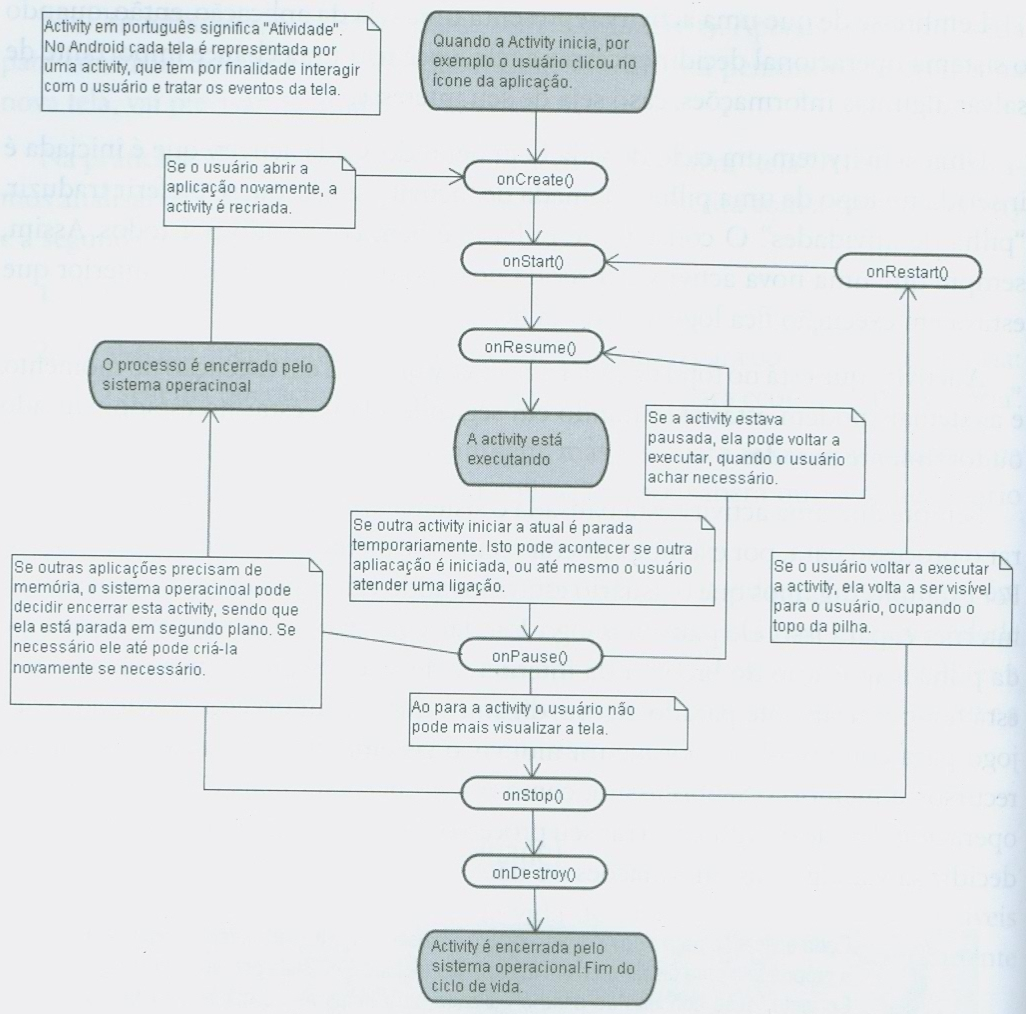
\includegraphics[width=10cm]{img/android_lecheta}
    \caption{Ciclo de vida de uma activity (Fonte: \cite{lecheta})}
    \label{Activity_lifecycle}
\end{figure}

Todos os métodos apresentados na Figura \ref{Activity_lifecycle} são métodos 
da classe Activity, que deverão ser sobrescritos pelas aplicações, e a chamada a esses
métodos ficara a cargo do sistema operacional.

Além desses métodos há um outro importante método automaticamente executado e de 
grande importância do que diz respeito a salvar o estado atual da aplicação: 
{\it onSaveInstanceState(Bundle)}. Este método é executado antes da atividade entrar em 
background, permitindo que seja salvo estado dinâmico em um objeto {\it Bundle}, para depois 
ser recuperado em {\it onCreate(Bundle)}, se a atividade precisa ser recriada. No entanto,
em relação a dados persistentes é necessário que eles sejam salvos no método {\it onPause()}, 
já que o {\it onSaveInstanceState(Bundle)} não faz parte do ciclo de vida, não sendo chamado 
em todas as situações.

% ------------------------------------------------------------------------------
\section{Estudo de caso: Froid - Fortunes for Android}

Como estudo de caso, utilizamos uma aplicação disponibilizada por \cite{abp}, a 
Froid - Fortunes por Android. Essa aplicação visa disponibilizar um widget que 
mostre frases aos usuários, sendo possível buscar mais frases na Internet. 

Com base na documentação disponibilizada, definimos uma versão preliminar do feature 
model da aplicação, apresentado na Figura \ref{fortunes_fm}. Quando possível, utilizaremos
esta aplicação como exemplo para os conceitos apresentados.

\begin{figure}[h]
    \centering
    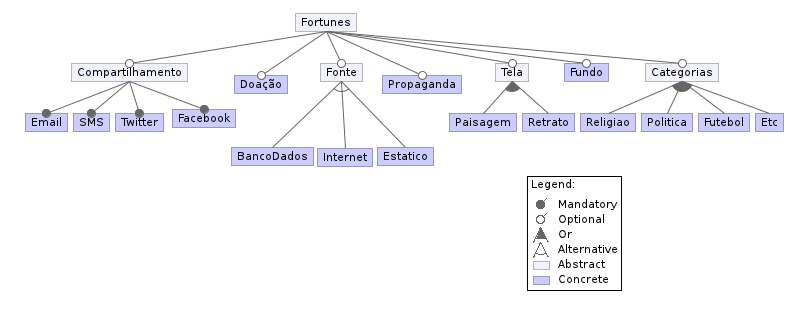
\includegraphics[width=10cm]{img/fortunes_fm}
    \caption{Feature model da aplicação Froid}
    \label{fortunes_fm}
\end{figure}



Um dos elementos de variação mais óbvios nos dispositivos móveis é o tamanho das telas.
Além disso, os aparelhos podem estar na posição vertical ou retrato, e, idealmente, 
as aplicações devem se adequar corretamente, aproveitando os espaços disponíves, ou 
adequando-se ao pouco espaço. O Android já fornece um mecanismo de layout relativo,
e como a interface do Froid é bastante simples, não foi necessário a definição de 
mais de um layout, no entanto, foi necessário implementar o {\it onSaveInstanceState(Bundle)}
para que quando o usuário rotacionasse o dispositivo, a frase exibida não fosse alterada, 
conforme exibido na Figura \ref{onSaveInstanceState}

\begin{figure}[h]
    \centering
    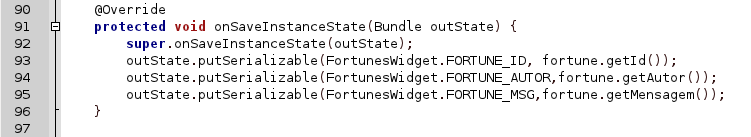
\includegraphics[width=10cm]{img/onSaveInstanceState}
    \caption{Método {\it onSaveInstanceState(Bundle)} da aplicação Froid}
    \label{onSaveInstanceState}
\end{figure}


% ..............................................................................
\section{Pontos de variações em dispositivos com Android}

Nessa seção, apresentaremos os pontos de variação em dispositivos com Android,
quando possível apresentaremos um exemplo com a aplicação Froid ou a de Times(?????)

\subsection{Versão da API}

A primeira versão da API do Android foi disponibilizada em outubro de 2008. De lá 
para cá, ele vem passando por diversas modificações, sendo a maioria deles ou 
introdução ou substituições de funcionalidades. Como partes da API são autualizadas, 
as partes antigas são marcadas como obsoletas e não removidas, assim aplicações feitas
com versões antigas da API continuarão funcionando nas mais recentes.

As versões da API são identificadas por um valor inteiro único chamado de {\it API Level},
distribuidas juntamente com as versões da plataforma Android. A Figura \ref{api_level} 
apresenta a relação entre versão da plataforma e {\it API Level}, além da distribuição.

\begin{figure}[h]
    \centering
    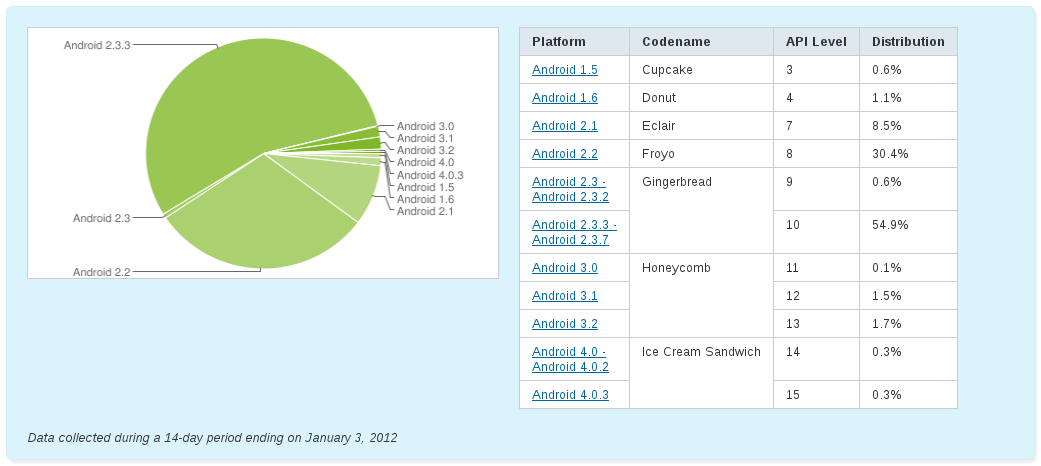
\includegraphics[width=15cm]{img/api_level}
    \caption{Distribuição da versão da plataforma e API Level (Fonte: \cite{platform_versions}) }
    \label{api_level}
\end{figure}

\subsection{Tamanhos e densidade das telas}

O Android executa em uma grande variedade de dispositivos, com diferentes tamanhos
 de telas e densidades. Para facilitar o projeto de interface para diferentes 
 configurações, a plataforma divide os atuais intervalos de tamanhos de telas e
 densidades em grupos, conforme abaixo:
\begin{itemize}
    \item Tamanhos de tela: small, normal, large, e xlarge
    \item Densidades: ldpi (low), mdpi (medium), hdpi (high), e xhdpi (extra high)
\end{itemize}
 
A Figura \ref{intervalos_telas} ilustra como os diferentes tamanhos de telas 
(em polegadas) e 
densidades (em dpi) são categorizados nesses diferentes grupos.

\begin{figure}[h]
    \centering
    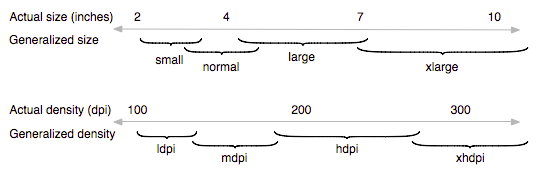
\includegraphics[width=15cm]{img/intervalos_telas}
    \caption{Relação entre tamanhos de telas e densidades e seus respectivos grupos 
        (Fonte: \cite{sup_multi_screens}) }
    \label{intervalos_telas}
\end{figure}

A Figura \ref{distribuicao_telas} apresenta a distribuição atual de tamanhos 
de tela e densidade.

\begin{figure}[h]
    \centering
    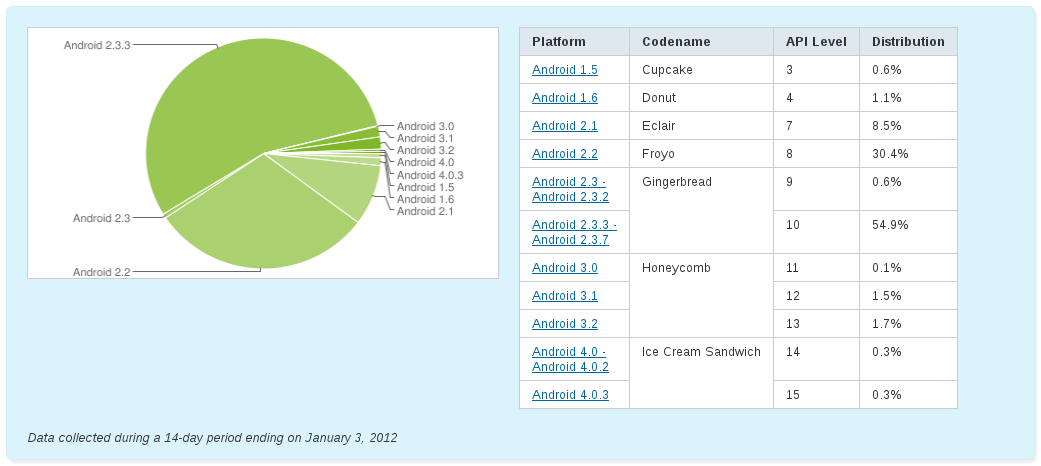
\includegraphics[width=15cm]{img/api_level}
    \caption{Distribuição atual de tamanhos de tela e densidades (Fonte: \cite{sup_multi_screens})}
    \label{distribuicao_telas}
\end{figure}


\subsection{Versão da OpenGL ES}

O Android oferece suporte para gráficos otimizados através de uma biblioteca 2D 
customizada. Quando suportado pelo hardware do dispositivo, gráficos 3D serão 
providos pela biblioteca OpenGL ES. A Figura \ref{distribuicao_opengl} apresenta 
a distribuição atual de versões dessa biblioteca encontradas nos aparelhos.

\begin{figure}[h]
    \centering
    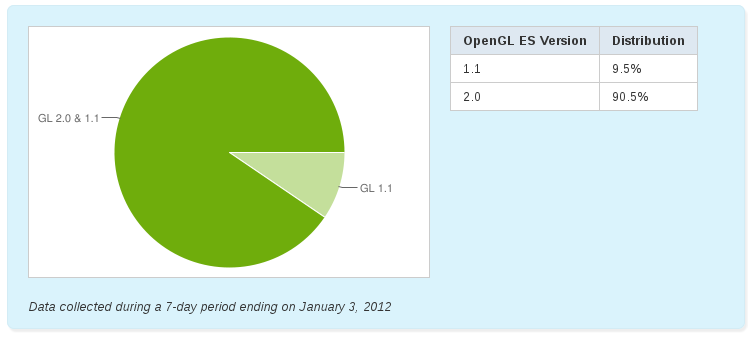
\includegraphics[width=15cm]{img/opengl}
    \caption{Distribuição atual da OpenGL ES (Fonte: \cite{opengl_versions})}
    \label{distribuicao_opengl}
\end{figure}


\subsection{Hardware e sensores do dispositivo}

Android oferece suporte para diversos tipos de sensores e hardware presentes nos 
dispositivos. Contudo, nem todos os dispositivos terão todos os tipos de sensores.
Incluem-se aqui, os mecanismos de interação do usuário com o aparelho.
Sensores e hardware que poderão ou não estar presentes nos dispositivos incluem:
\begin{itemize}
    \item Acelerômetro
    \item Câmera
    \item Sensor de luminosidade
    \item Bluetooth
    \item Wifi
    \item Live wallpaper
    \item GPS
    \item Microfone
    \item Sensor de proximidade
    \item Telefone VoIP baseado em SIP
    \item Telefonia CDMA e/ou GSM
    \item USB
    \item Mecanismos de interação
    \begin{itemize}
        \item Tela sensível a toque e/ou multitoque
        \item Teclado físico
        \item Trackball
        \item Botões de navegação (five-way navigation pad)
    \end{itemize}
\end{itemize}


\subsection{Línguas internacionais}
Os textos das mensagens no sistema operacional costumam estar no idioma nativo do usuário.
É desejável que os textos das aplicações também estejam nesse mesmo idioma, e que 
isso seja possível de forma transparente para o usuário.

% ..............................................................................
\section{Mecanismos de controle de variabilidades}

Nessa seção, discutiremos os mecanismos fornecidores na plataforma Android que 
poderão ser utilizados para tratar os diversos pontos de variações apresentados.

\begin{itemize}
    \item Polimorfismo
    \item Reflexão
    \item Classe wrapper
    \item Checagens de versão da API e de recursos do aparelho em tempo de execução
    \item Atributos final e Compilação Condicional 
    \item Recursos da Aplicação
    \item Android NDK
    \item Pacote de compatibilidade
\end{itemize}

% ..............................................................................
\subsection{Polimorfismo}

Conforme pode ser observado na Figura \ref{fortunes_fm}, a origem das frases do 
Froid pode ser um banco de dados local ou a Internet, através de um web-service.
Essa distinção foi feita através da implementação de uma interface Java: 
{\it FortuneProvider}.
Para cada tipo de fonte, foi feita uma implementação dessa interface: 
{\it FortuneProviderDatabase} para o banco de dados e {\it FortuneProviderService} para webservice. 
Além desses, analisando o código fonte foi identificado uma terceira fonte de dados, 
{\it FortuneProviderStatic}, que contém frases definidas estaticamente no código, e é 
utilizada para testes das demais funcionalidades da aplicação.

\begin{figure}[h]
    \centering
    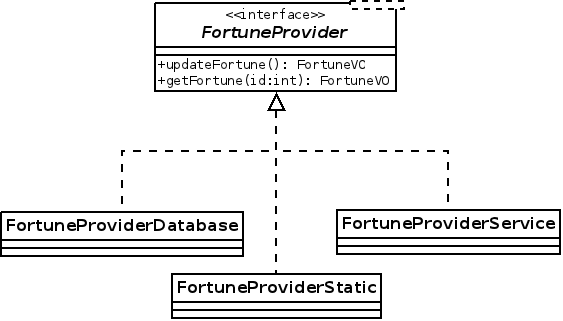
\includegraphics[width=10cm]{img/implementacao_FortuneProvider}
    \caption{Diagrama de classes, mostrando a interface e suas implementações}
    \label{diagrama_classes}
\end{figure}

A fim de facilitar a instanciação dos providers, foi definido uma classe 
instanciadora, {\it FortuneProviderUtils}, apresentada na Figura \ref{provider_utils}.
Na Figura \ref{instanciando_provider}, podemos ver essa classe sendo utilizada para 
instanciar um provider. Sendo que a definição da fonte, se será banco de dados, 
webservice ou estático é feita de forma manual, durante a compilação.

\begin{figure}[h]
    \centering
    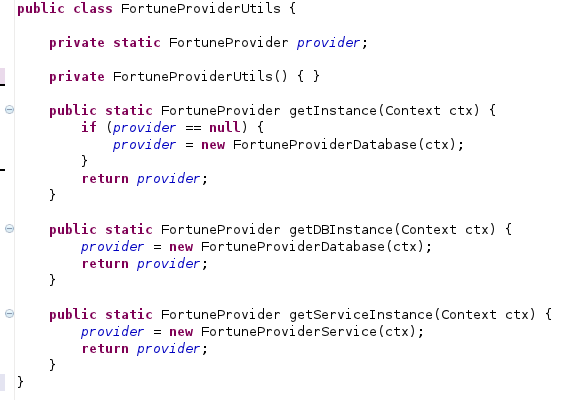
\includegraphics[width=10cm]{img/FortuneProviderUtils}
    \caption{Classe FortuneProviderUtils}
    \label{instaciando_provider}
\end{figure}

\begin{figure}[h]
    \centering
    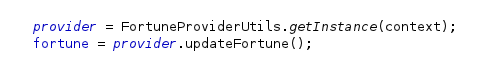
\includegraphics[width=10cm]{img/instaciando_provider}
    \caption{Instanciando um provider em específico}
    \label{instaciando_provider}
\end{figure}

% ------------------------------------------------------------------------------

\subsection{Compatibilidade com versões antigas da API}

A API do Android evolui oferecendo novos recursos para os desenvolvedores utilizarem.
No entanto, eles também desejam que suas aplicações continuem executando em 
dispositivos com versões anteriores, sem o novo recurso.

Isso será possível para recursos não essenciais, como um virtual mesmo que um teclado físico esteja disponível. Então você poderá escrever sua aplicação para usar o novo 
recurso sem que ela falhe em dispositivos antigos. Há duas formas para atingir esse objetivos, discutidos a seguir.

\subsubsection{Reflexão}

Suponha que se deseje utilizar um novo método, introduzido em nova versão da API,
como {\it android.os.Debug.dumpHprofData(String filename)}. A classe {\it android.os.Debug}
já existia desde a primeira versão do SDK, mas o método foi adicionado somente na versão 
1.5, se você acessá-lo diretamente, sua aplicações irá falar em dispositivos antigos.

A maneira mais simples para chamar o método é através de reflexão. Será feita uma 
verificação se o método existe, e o resultado será armazenado em um objeto {\it Method}.
Quando for necessário o método ser executado, isso será feito através de 
{\it Method.invoke}. Considere a Figura \ref{class_reflect1}:

\begin{figure}[h]
    \centering
    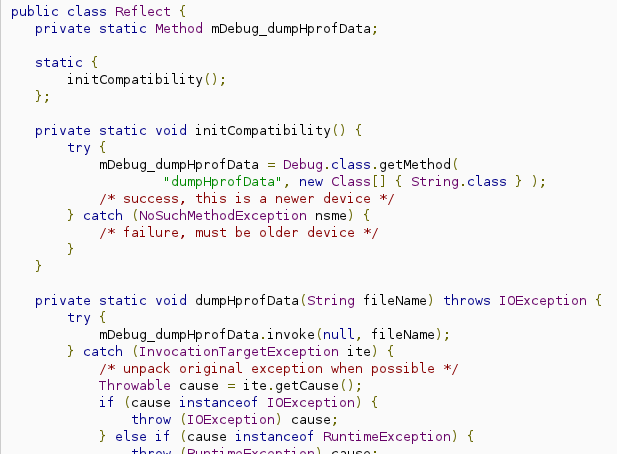
\includegraphics[width=10cm]{img/reflect1}
    \caption{Trecho da classe Reflect onde é verificado se o método existe (Fonte \cite{back_compat})}
    \label{class_reflect1}
\end{figure}

A Figura \ref{class_reflect1} mostra que o método {\it initCompatibility} é executado
 estaticamente e é responsável por verificar se o método existe. Se sim, usa um método 
 privado com a mesma assinatura do original para poder chamá-lo. 

\begin{figure}[h]
    \centering
    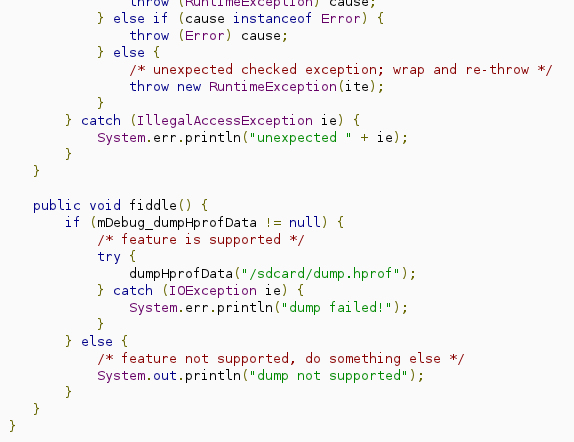
\includegraphics[width=10cm]{img/reflect2}
    \caption{Trecho da classe Reflect onde o método é executado (Fonte \cite{back_compat})}
    \label{class_reflect2}
\end{figure}

A Figura \ref{class_reflect2} demostra como a aplicação pode escolher entre chamar 
a nova API ou fazer algo diferente baseado na existência ou não do novo método.

Para cada método adicional que você queira executar, deverá adicionar um atributo 
{\it Method}, um atributo inicializador, e um empacotador da chamada para a classe.

Essa abordagem ficará complexa quando o método está declarado em um classe que não 
existia anteriormente. Além disso, chamar {\it Method.invoke()} será mais lento 
que invocar o método diretamente. Esses problemas podem ser diminuídos usando uma
classe empacotadora.

% ..............................................................................
\subsubsection{Classe empacotadora}

A ideia é criar uma classe que empacota toda a nova classe. Cada método na classe 
empacotadora (wrapper) apenas executa o método real correspondente, repassando os 
parâmetros, e retorna o mesmo resultado.

Se a classe alvo e o método existem, você irá ter o mesmo comportamento que teria se 
executasse a classe diretamente. Se a classe ou método não existem, a inicialização
da classe empacotadora falha, e sua aplicação sabe que deverá evitará usar os novos 
métodos.

Suponha que a classe apresentada na Figura \ref{wrapper1} seja uma nova classe adicionada.
Nós deveremos criar uma classe empacotadora para ele, apresentada na Figura \ref{wrapper2}.

\begin{figure}[h]
    \centering
    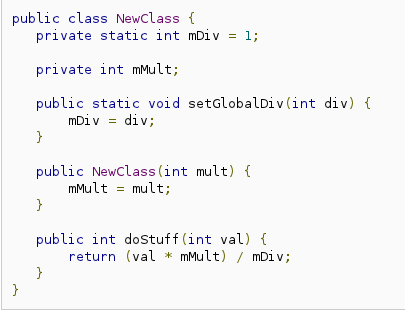
\includegraphics[width=10cm]{img/wrapper1}
    \caption{Nova classe (Fonte: \cite{back_compat})}
    \label{wrapper1}
\end{figure}

\begin{figure}[h]
    \centering
    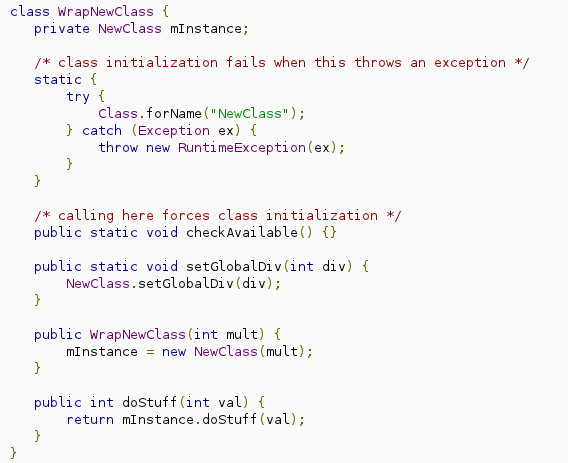
\includegraphics[width=10cm]{img/wrapper2}
    \caption{Classe empacotadora (Fonte: \cite{back_compat})}
    \label{wrapper2}
\end{figure}

A classe empacotadora tem um método para cada construtor e cada método no original,
mais uma inicializador estático que testa se a nova classe existe. Se a nova classe
não está disponível, a inicialização de {\it WrapNewClass} irá falhar, assegurando
que classe empacotadora não seja utilizada indevidamente. O método {\it checkAvailable} 
é usado como um meio simples para forçar a inicialização da classe. A Figura \ref{wrapper3}
mostra como isso deverá ser utilizado.

\begin{figure}[h]
    \centering
    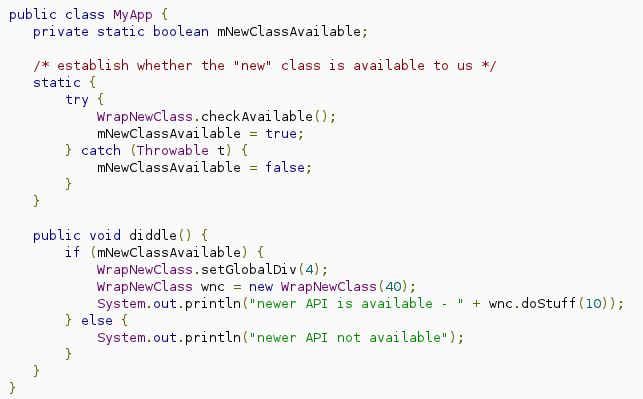
\includegraphics[width=10cm]{img/wrapper3}
    \caption{Utilizando a classe empacotadora (Fonte: \cite{back_compat})}
    \label{wrapper3}
\end{figure}

Se a chamada para {\it checkAvailable} for feita com sucesso, saberemos que a nova
classe faz parte do sistema. Se falar, saberemos que ela não está presente, então
poderemos ajustar a execução da aplicações de acordo com isso.

% ..............................................................................
\subsection{Checagem da versão da API em tempo de execução}

Texto + imagens dos slides 26

% ..............................................................................
\subsection{Checagem da existência de um determinado recurso}
Pode-se utilizar o método PackageManager.hasSystemFeature() para determinar se o 
dispositivo possi um determinado recurso

% ..............................................................................
\subsection{Atributos com modificadores final}

Texto + imagens dos slides 28


% ..............................................................................
\subsection{Compilação condicional}

Texto + imagens do slide 29


% ..............................................................................
\subsection{Recursos da aplicação}

Texto + imagens dos slides 30-34


% ..............................................................................
\subsection{Compartilhamento de informações}

Texto + imagens dos slides 25

